\documentclass{article}

\usepackage{listings}
\usepackage{graphicx}
\usepackage{hyperref}
\usepackage{fancyref}

\title{A Novel Type-Independent Sorting Algorithm}
\author{Cole Kurashige \\ Harvey Mudd College}
\date{2020 \\ March}

\begin{document}

\section{Abstract}
This section is abstract.

\section{Background}
Lower bounds for time and space complexity have been long-established for
comparison-based sorting algorithms. Many sorting algorithms have been developed
which vary in the trade-offs they make for these complexities. Little has been
done, however, to examine what it means to make a comparison.

In statically-typed programming languages like Java or C++, comparisons such as
equal to (\texttt{==}) or greater than (\texttt{>}) are often restricted to
operating on two elements of the same type\footnote{At least, without trickery
  or custom comparators.}. These languages consider it a compliation error
to compare elements of differing types.

Dynamically-typed programming languages like Python do not consider it a
compilation error; however, it is usually a runtime error to make these
comparisons.

\begin{lstlisting}[caption = Comparisons in Python 3.7.6]
>>> -1 > '-2'
Traceback (most recent call last):
  File "<stdin>", line 1, in <module>
TypeError: '>' not supported between instances of 'int' and 'str'
\end{lstlisting}

JavaScript, ever the staunch opponent of reason, will gladly compare two objects
of differing types. But just because JavaScript can do something does not mean
that JavaScript does it right.

It will correctly report that \texttt{-1} is greater than \texttt{"-2"}, but it
erroneously considers \texttt{"-1"} less than \texttt{"-2"}. It also doesn't get
that \texttt{"three"} is less than \texttt{"four"}, and it certainly does not
know that \texttt{"one pound of feathers"} is just as heavy as \texttt{"one
  pound of bricks"}.

\begin{lstlisting}[caption = Comparisons in JavaScript (Node.js 12.12.0)]
> -1 > "-2"
true
> "-1" > "-2"
false
> "three" < "four"
false
> "one pound of feathers" == "one pound of bricks"
false
\end{lstlisting}

Though it would be enjoyable to continue to mock JavaScript and its many
questionable design choices, we cannot fault much for these shortcomings.

JavaScript, like any programming language, interprets code. It treats queries
like \texttt{"-1" > "-2"} as being a comparison on characters, not numbers, even
if we humans can plainly see that JavaScript is being asked to compare negative
one and negative two. But we cannot call JavaScript an idiot without calling it
a savant. It can perform remarkably complex calculations in the blink of an eye
or bring the fastest of hardware to a slow grind.

Computers are limited at processing much of the information that is so easy for
us humans to immediately understand, like pictures of dogs or whether
\texttt{"-1"} is greater than \texttt{"-2"}. And we are limited at processing
much of the information that is so easy for computers, like the exact colors of
the millions of pixels in a picture of a dog or the product o two very large
numbers.

\begin{lstlisting}[caption = Complex Operations in JavaScript (Node.js 12.12.0)]
> 0.1 + 0.2
0.30000000000000004
> 1000000000 * 500000000
500000000000000000
\end{lstlisting}

Together, computers and humans can cover for each others' inadequacies, which is
the premise of Human-Computer Interaction. Human-Computer cooperation has yet to
be fully realized in sorting algorithms, which have focused on maximizing
computational performance. At least until now.

\section{Turksort}

The idea behind turksort is simple: let computers handle all of the sorting
tedium and let humans handle all of the comparisons. In that regard, turksort is
not that different from most sorting algorithms.

All of the sorting remains the same, except whenever a request for a comparison
between two values is made, a form is generated. This form asks which of the two
is greater\footnote{``Neither'' is an option, too.}. The form is sent to
Amazon's Mechanical Turk\footnote{\url{https://www.mturk.com/}} where a worker
(known as a ``turker'') fills it out. The answers is sent back and then used
for the comparison. \Fref{fig:comparison} depicts this process.

A sample implementation of Turksort is available at \url{}.

\begin{figure}
  \centering
  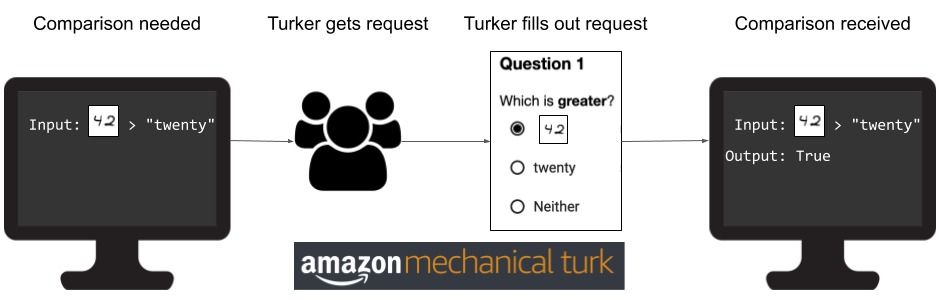
\includegraphics[width=300pt]{diagram-1.png}
  \caption{How Turksort comparisons work}
  \label{fig:comparison}
\end{figure}

\end{document}